\chapter{データセット}
\label{chap:dataset}
\fancyhf{}
\rhead{\thepage}
\lhead{第\ref{chap:dataset}章 データセット}
\cfoot{\thepage}


本章では,
実験で用いるデータセットについて述べる.
データセットは,小学4年生から中学3年生を対象とする国内最大級のMOOCs「勉強サプリ\footnote{\url{https://benkyosapuri.jp/}}」で提供される11の講座の問題回答ログデータから作成する
\footnote{本論文の研究は勉強サプリを運営するリクルートマーケティングパートナーズ(株)との共同研究プロジェクトの一環で行われている.}
.
まず,勉強サプリから収集されたログデータが分析に利用するためのデータ要件を満たした本分析に最適なデータであることを述べる.
次に,実験で用いる宣言的知識の獲得を主目的とするデータセットと手続き的知識の獲得を主目的とするデータセットの作成について述べる.
特に,
歴史や地理に関する講座の問題が主に宣言的知識の獲得の有無を評価する問題であることを指摘し,
歴史や地理に関する5講座から宣言的知識の獲得を主目的とするデータセットとして5つのデータセットを作成する.
また,
算数や数学に関する講座の問題が主に手続き的知識の獲得の有無を評価する問題であることを指摘し,
算数や数学に関する6講座から手続き的知識の獲得を主目的とするデータセットとして6つのデータセットを作成する.






\section{勉強サプリ}
ここでは,勉強サプリより収集された問題回答ログデータが本分析に最適なデータであることを述べるため,
まず,勉強サプリについて説明する.
% - 勉強サプリは5W1H(what, who, when, where, why, how)
勉強サプリは主に小学4年生から中学3年生を対象とした国内最大級の大規模オンライン講座である.
リクルートマーケティングパートナーズ(株)が運営している.
サービスは2015年に開始された.
学習者はオンライン上で問題回答形式によるドリル演習や
動画視聴形式による授業聴講を通して勉強する.
小学生には各学年ごとに国語,社会,算数,理科の4科目が,
中学生には各学年ごとに国語,数学,英語の3科目と 
学年共通で地理,歴史,公民,理科1,理科2の5科目が提供されており
合計26の講座が提供されている.
%フリーミアム形式で提供されており,
無料で利用できるコンテンツもある.



% - 統計量
勉強サプリは提供教材,利用者数,学習行動ログ数の点でサービスの規模が非常に大きい.
4,000以上の授業動画と7,000近い演習問題を提供しており,
サービス開始から1年経たずして,
利用者は5万人以上おり,
講義視聴ログ数は100万以上,
問題回答ログ数は総計で1,000万以上である\footnote{2015年11月31日時点.}.


% - 利用画面
\begin{figure}[!htb]
\begin{center}
	\hspace*{-10pt}\makebox[1.2\textwidth][c]{
		\minipage{0.52\textwidth}
			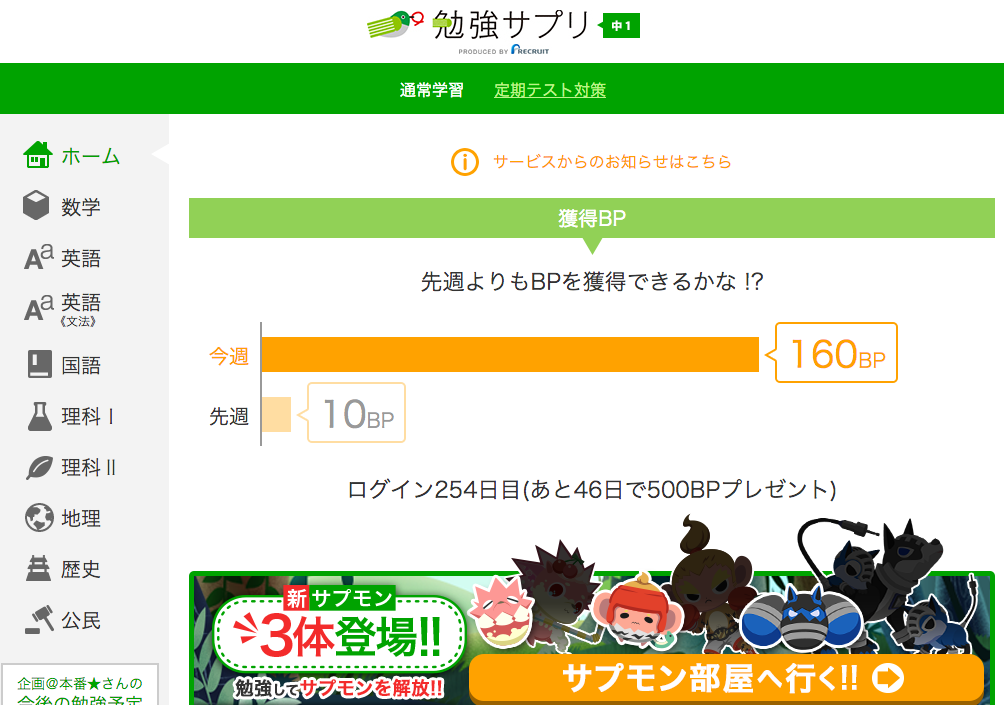
\includegraphics[width=200pt, height=160pt]{./img/benkyo1.png}
			\caption{勉強サプリのマイページ}
			\label{fig:benkyo1}
		\endminipage\hfill
		\minipage{0.52\textwidth}
			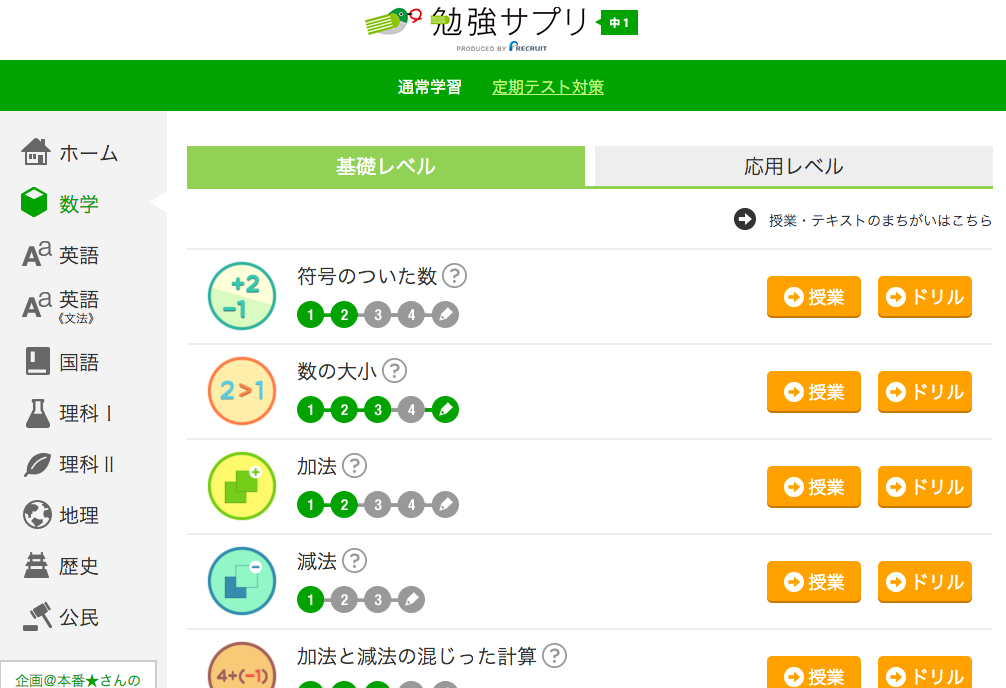
\includegraphics[width=200pt, height=160pt]{./img/benkyo2.png}
			\caption{勉強サプリの講義一覧ページ}
			\label{fig:benkyo2}
		\endminipage\hfill
	}
	\hspace*{-10pt}\makebox[1.2\textwidth][c]{
		\minipage{0.52\textwidth}
			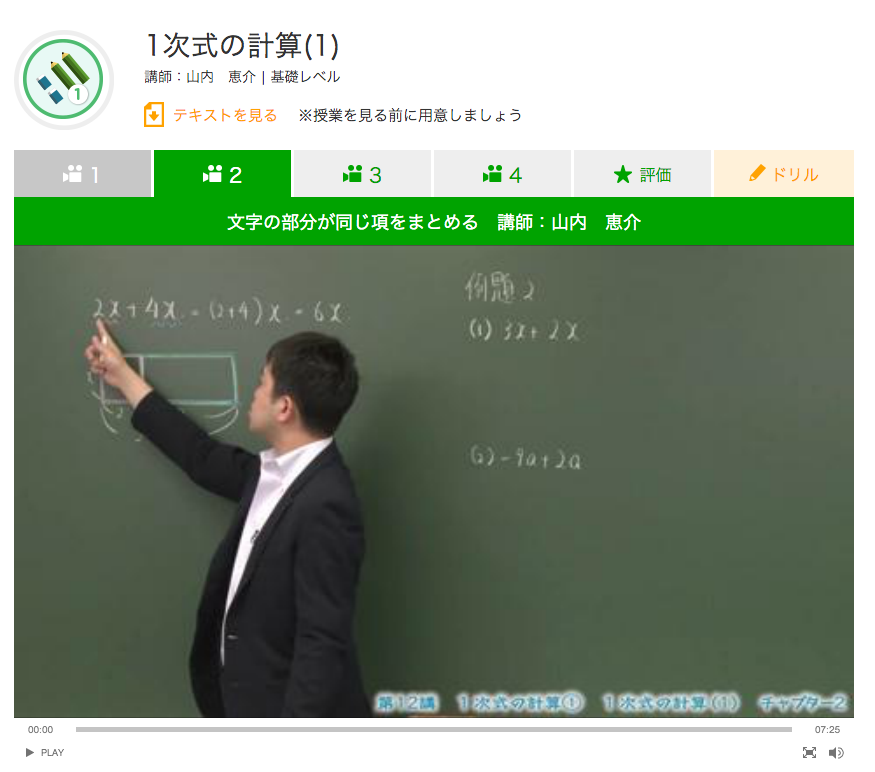
\includegraphics[width=200pt, height=160pt]{./img/benkyo3.png}
			\caption{勉強サプリの講義視聴ページ}
			\label{fig:benkyo3}
		\endminipage\hfill
		\minipage{0.52\textwidth}
			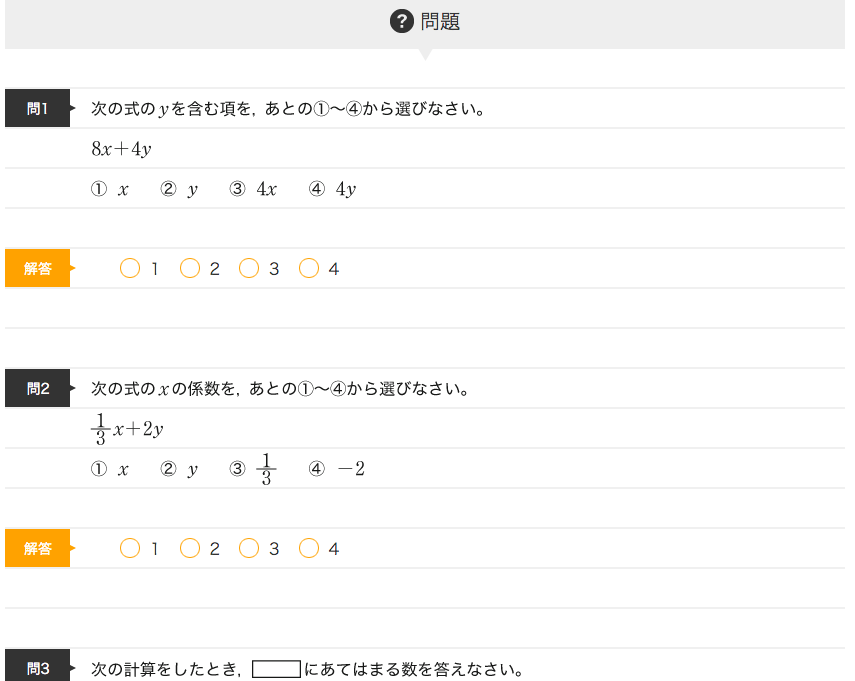
\includegraphics[width=200pt, height=200pt]{./img/benkyo4.png}
			\caption{勉強サプリの問題演習ページ}
			\label{fig:benkyo4}
		\endminipage\hfill
	}
\end{center}
\end{figure}
サービスの具体を利用画面を交えて説明する.
図\ref{fig:benkyo1},\ref{fig:benkyo2},\ref{fig:benkyo3},\ref{fig:benkyo4}にページのイメージを記載する.
図\ref{fig:benkyo1}はログイン後のマイページを示している.
学習に関するコンテンツだけでなく,
利用継続性の向上を狙って,ポイントというシステムやサプモン(勉強サプリのモンスター)というアバターを用いたゲームを大きく表示している.
図\ref{fig:benkyo2}は中学1年向け数学の講義一覧ページを示している.
ユーザは講義視聴のドリル演習の両方あるいはどちらかを勉強できる.
図\ref{fig:benkyo3}は講義視聴ページを示している.
講義視聴ページは視聴しやすいように細かく分割されている.
図\ref{fig:benkyo4}は問題演習ページを示している.
問題演習はテスト形式で提供されており,一度に複数の問題が提供され,また,その採点も同時に行われる.
この問題回答から収集されるログデータの仕様は同時に1つの問題しか回答ログが入らないというDeep Knowledge Tracingで想定されている設定と異なるため,
Deep Knowledge Tracingを拡張する必要があるが,その拡張法については実験説明の際に合わせて述べる.


現在の学習指導要領\cite{gakushushidouyouryou}によると,
小学4年生の社会では社会基盤や地域社会など地理に近い内容を扱い,
小学5年生の社会では地域の山地山脈,気候など地理に近い内容を扱い,
小学6年生の社会では日本の歴史に関する内容を扱う
としており,
また,実際に,勉強サプリの学習内容も概ねそれに従っている.


勉強サプリは小学生から中学生が対象で,
その難易度は難しすぎず,
収集された問題回答ログデータは1,000万以上と膨大であり,
また,先に指摘したような地理や歴史といったいわゆる暗記系の科目と数学に関する科目が複数提供されているため,
データの要件を満足している可能性が高い.
そこで,
以降では,勉強サプリから収集された問題回答ログデータのなかで,
特に地理と歴史に関する5講座(小学4年社会,小学5年社会,小学6年社会,中学地理,中学歴史)のデータ
と,
算数や数学に関する6講座(小学4年算数,小学5年算数,小学6年算数,中学1年数学,中学2年数学,中学3年数学)のデータ
の11データよりデータセットを作成し,
これらのデータセットを
それぞれ,
宣言的知識の獲得を主目的とするデータセットと手続き的知識の獲得を主目的とするデータセットとする.


\section{データセットの作成}
データセットの作成について述べる.
データセットは問題回答ログデータから作成する.
対象期間は2015年4月から2015年11月の8ヶ月である.

勉強サプリでは学習者の回答は自動採点される.いずれの講座も回答は選択方式で,1つの回答欄には選択肢の中から1つの数字や文字を選択する.
1つの問題に複数の回答欄が存在する場合は当該問題のすべての回答欄が正解の場合に当該問題を正解した,と扱う.同時に1つの問題しか提示されないという形式だけでなく,同時に複数の問題が提示される場合もあり,その場合,採点は提示された問題群に対して同時に行われる.つまり,同時に複数の問題回答ログが発生しうるデータである.

データセットを作成する際に,前処理として回答行動ログデータから下記に該当するログデータをノイズとみなして除去した.
\begin{itemize}
	\item[条件] 同時に回答された複数の問題のログデータ群について,すべての問題の回答欄が空白で投稿されているもの.
\end{itemize}
これは,オンライン講座ではサービス上の学習者の行動には大きな制約はなく,
1クリックで簡単に問題演習ページを開けてしまえる状況にあるということや,
すべての回答欄が未記入で投稿された回答は直前に着手した問題群と同じ問題群であることが多いこと,
特に回答時間が短く誤って当該問題演習ページを開いてしまったと推察されるログが多かったからである.

以上,データセットの作成について述べた.
11データセット全体を概観する.

\section{データセットの概観}
\begin{table}[!htb]
\caption{11データセットの統計量}
\label{tab:datasets-overview}
\begin{center}
\centerline{
{
\begin{tabular}{cc|rrrrr}\hline\hline
\multirow{2}{*}{学年}&	\multirow{2}{*}{科目}	&	\multirow{2}{*}{ユーザ数}	&	\multirow{2}{*}{問題数}		&	\multirow{2}{*}{回答ログ数}		&	\multirow{2}{*}{\shortstack{回答ログ数\\ $\div$ユーザ数}}	&		\multirow{2}{*}{\shortstack{回答ログ数\\ $\div$問題数}}		\\
				&								&								&								&									&				&			\\\hline
\multirow{2}{*}{小学4年}&		社会			&	3,045						&	76							&	227,409			&	75							&	2,992	\\	
				&				算数			&	4,318						&	182							&	505,917			&	117							&	2,780	\\\hdashline	
\multirow{2}{*}{小学5年}&		社会			&	2,833						&	197							&	388,521			&	137							&	1,972	\\	
				&				算数			&	3,380						&	257							&	411,957			&	122							&	1,603	\\\hdashline	
\multirow{2}{*}{小学6年}	&	社会			&	2,891						&	202							&	434,324			&	150							&	2,150	\\	
				&				算数			&	3,225						&	245							&	395,276			&	123							&	1,613	\\\hdashline	
中学1年			&				数学			&	7,137						&	365							&	659,237			&	92							&	1,806	\\	
中学2年			&				数学			&	3,931						&	278							&	238,241			&	61							&	857	 	\\   
中学3年			&				数学			&	2,667						&	343							&	177,295			&	66							&	517	 	\\\hdashline   
\multirow{2}{*}{中学}&			地理			&	6,499						&	308							&	660,882			&	102							&	2,146	\\	
				&				歴史			&	6,381						&	364							&	853,419			&	134							&	2,345	\\	
\hline\hline
\end{tabular}
}
}
\end{center}
\end{table}
作成した11データセットを概観する.
11データセットそれぞれについてユーザ数,問題数,回答ログ数とそれらの関係性を表\ref{tab:datasets-overview}に整理した.
それぞれについて順に説明していく.

まず,ユーザ数について, 
全体として,数千以上のユーザのログデータに基づいたものとなっており,最も差の大きい2つのデータセット(中学1年の数学と中学3年の数学)間で差は$2.6$倍程度である.
特に,ユーザ数が多いのは7,000ユーザ以上の中学1年の数学で,それに続いて,6,000ユーザ以上の中学の地理,歴史である.

次に,問題数について,
全体として,数十から数百の問題に基づいたものとなっており,最も差の大きい2つのデータセット(小学4年の社会と中学1年の数学)間で差は$4.8$倍程度である.
小学生のデータセットよりは中学生のデータセットの方が問題数が大きい傾向にあり,
特に,問題数が多いのは360以上の中学1年の数学と中学歴史である.

回答ログ数については,
全体として,
数十万以上であり, 最も差の大きい2つのデータセット(中学歴史と中学3年の数学)間で差は$4.8$倍程度である.
特に回答ログ数が最も大きい中学歴史のデータセットは85万以上と大規模な問題回答ログデータからなる.

さらに,これら3つの統計量の関係性を捉えるために,ログの密度という観点からユーザ1人あたりの平均回答ログ数と問題1問あたりの回答ログ数の2つの指標を評価した.
まず,ユーザ1人あたりの平均回答ログ数について, 
全体として,数十から百数十となっており,最も差の大きい2つのデータセット(小学6年社会と中学2年数学)間で差は$2.5$倍程度である.
また,いずれのデータセットでも平均回答ログ数は問題数を下回っている.

次に,問題1問あたりの平均回答ログ数について, 
全体としては,数百から数千程度の値となっており,最も差の大きい2つのデータセット(小学4年社会と中学3年数学)間で差は$5.8$倍程度である.
特に,中学2年数学と中学3年数学が小さい傾向にある.
平均回答ログ数が最も大きい小学4年社会のデータセットは1問あたり3,000近いログデータが存在する.

以上,改めてデータセット間の各統計量について整理すると,
いずれのデータセットも非常に大規模な問題回答ログから構成されており,問題あたりのログ数という点でも十分を大きいと考えられる.
また,いずれの統計量もデータセット間においても10倍以上の開きはなく,
特に,ログ数の偏りによる今後の議論の影響は小さいと考えられる.


以上,11データセット全体を概観した.
次に,個々のデータセットを具体的に説明する.


\section{個々のデータセットの具体的説明}
本論文の対象である11データセットについて,それぞれのデータセットの性質について1つずつ述べる.
具体的には,
問題群の概要,
問題とその回答選択肢の具体例,
問題ごとの何番目に着手されるかの平均値と回答ログ数の関係
の3つである.
各問題について何番目に着手されるかの平均値は
各ユーザごとに当該講座の各問題を何番目に着手したかを算出し,
それらをユーザ全体で平均した値を用いる.
各問題について何番目に着手されるかの平均値と回答ログ数の関係を見ることで,
ユーザが講座の問題全体を均一に着手しているのか,もしくは,一部に偏っているのかを捉えることができる.
XYプロットとして可視化し,図のデータ点はそれぞれひとつの問題に相当する.

\subsubsection{小学4年社会}
\begin{figure}[ht]
\begin{center}
\minipage{0.48\textwidth}
	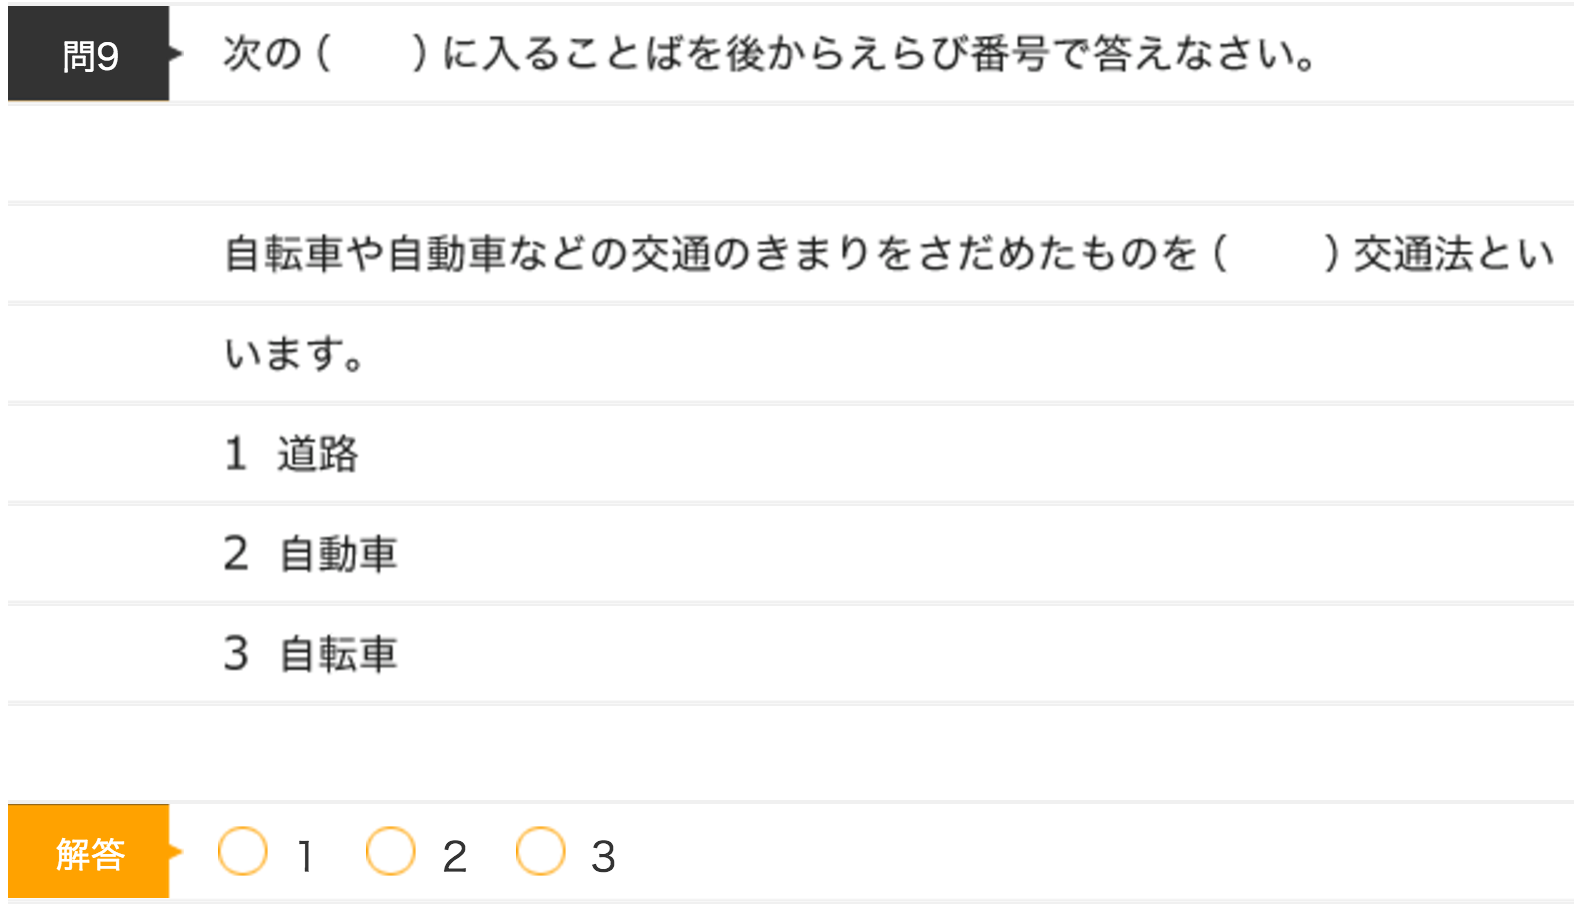
\includegraphics[width=200pt, height=150pt]{./img/qa_s4_soc.png}
	\caption{小学4年社会の問題と回答選択肢の例}
	\label{fig:qa_s4_soc}
\endminipage\hfill
\minipage{0.48\textwidth}
	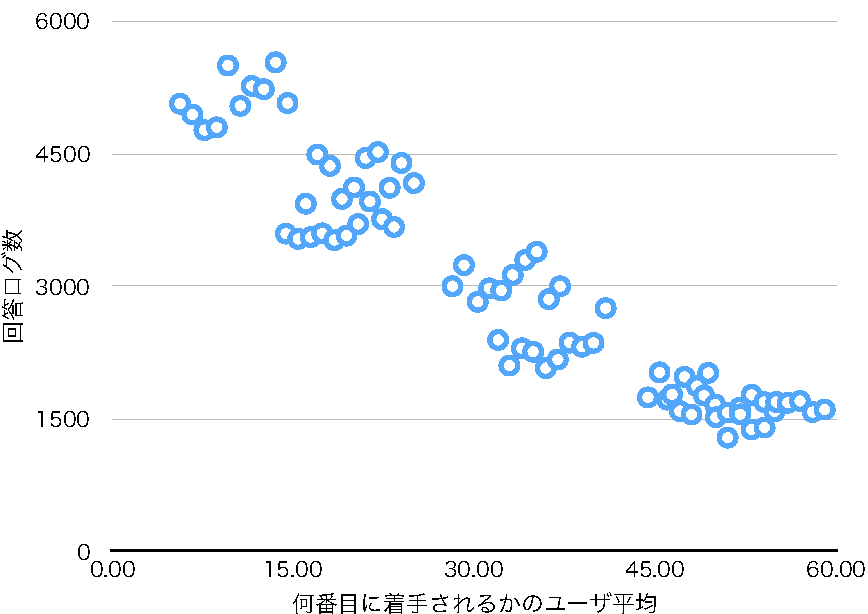
\includegraphics[width=200pt, height=150pt]{./img/stats_s4_soc.pdf}
	\caption{小学4年社会の平均着手順と回答ログ数のXYプロット}
	\label{fig:stats_s4_soc}
\endminipage\hfill
\end{center}
\end{figure}
小学4年社会では,主に,警察,消防,浄水場,ダム,汚水処理,発電所,ゴミ処理,リサイクル,水不足,地図の見方などの社会基盤や社会問題に関する基本内容が扱われる.
図\ref{fig:qa_s4_soc}に,問題と回答選択肢の例を示す.
図の問題は社会ルールのうち道路交通法に関する問題であり,
その回答を選択肢のなかから選択する,という回答形式である.
次に,各問題について何番目に着手されるかの平均値と回答ログ数の関係を図\ref{fig:stats_s4_soc}に示す.
全体として,概ね1500件以上の回答ログ数があり,最初の問題の方が回答ログが大きい傾向にあるが大きく偏っているというわけではない.



\subsubsection{小学4年算数}
\begin{figure}[ht]
\begin{center}
\minipage{0.48\textwidth}
	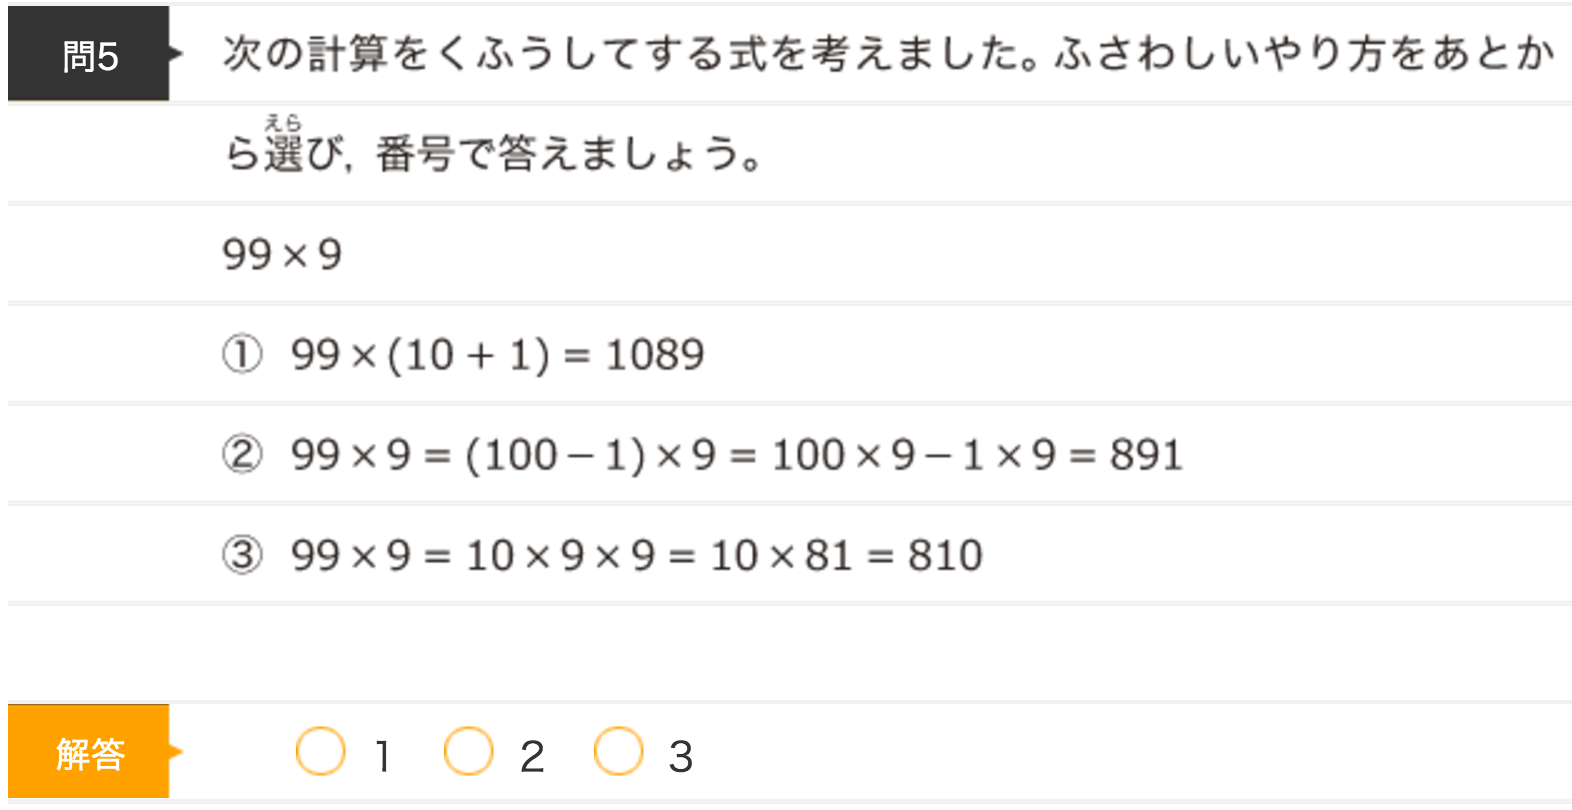
\includegraphics[width=200pt, height=150pt]{./img/qa_s4_mat.png}
	\caption{小学4年算数の問題と回答選択肢の例}
	\label{fig:qa_s4_mat}
\endminipage\hfill
\minipage{0.48\textwidth}
	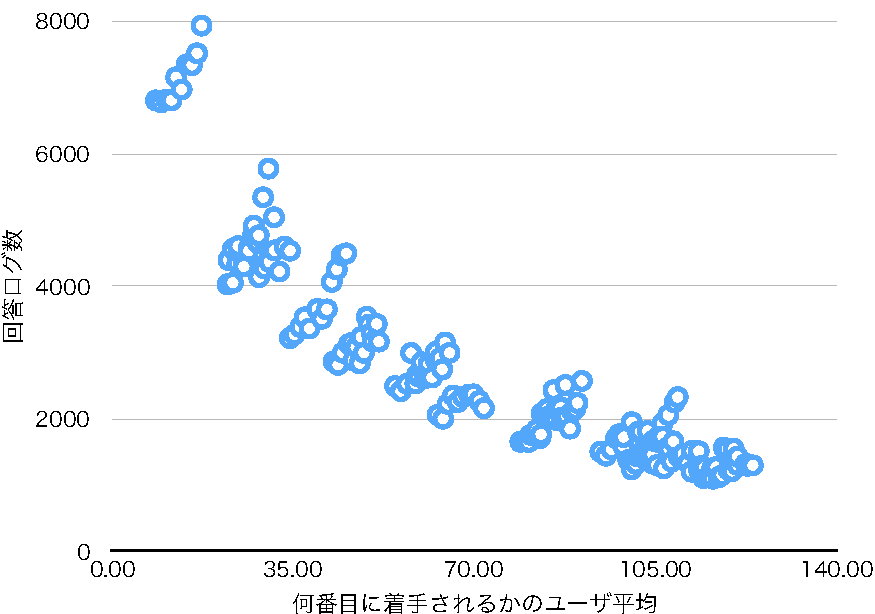
\includegraphics[width=200pt, height=150pt]{./img/stats_s4_mat.pdf}
	\caption{小学4年算数の平均着手順と回答ログ数のXYプロット}
	\label{fig:stats_s4_mat}
\endminipage\hfill
\end{center}
\end{figure}
小学4年算数では,主に,大きな数や小数など桁の認識,四則演算,数直線,折れ線グラフ,角度,分度器,垂直,並行,面積,単位,などの数理演算の基本内容が扱われる.
図\ref{fig:qa_s4_mat}に,問題と回答選択肢の例を示す.
図の問題は分配法則に関する問題であり,
その回答を選択肢のなかから選択する,という回答形式である.
次に,各問題について何番目に着手されるかの平均値と回答ログ数の関係を図\ref{fig:stats_s4_mat}に示す.
全体として,概ね1500件以上の回答ログ数があり,最初の問題の方が回答ログが大きい傾向にあるが大きく偏っているというわけではない.


\subsubsection{小学5年社会}
\begin{figure}[ht]
\begin{center}
\minipage{0.48\textwidth}
	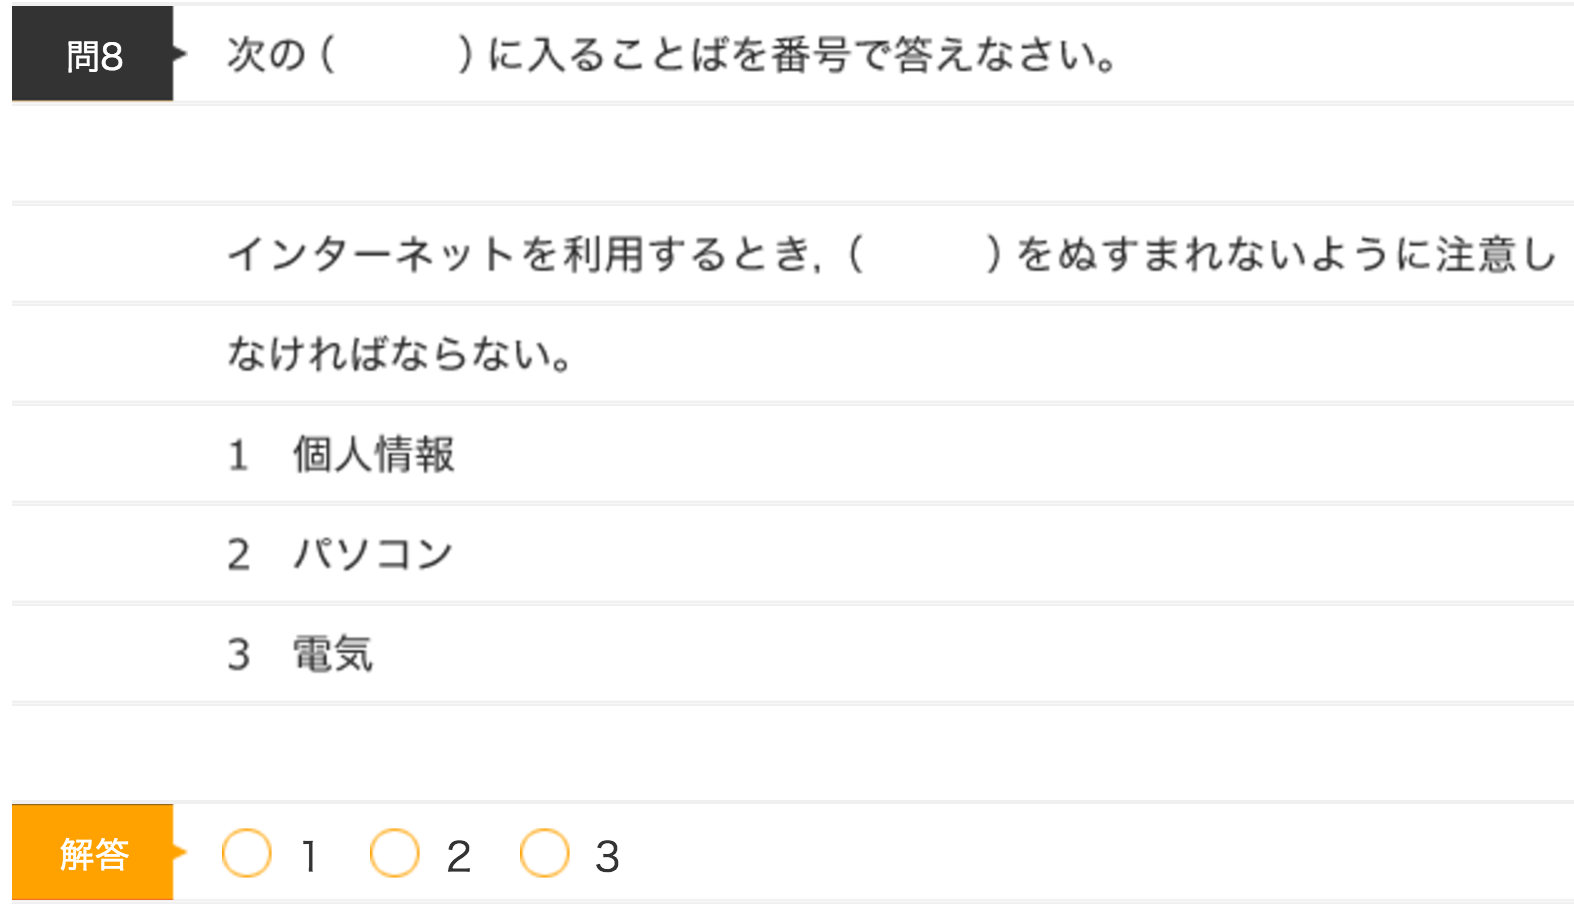
\includegraphics[width=200pt, height=150pt]{./img/qa_s5_soc.png}
	\caption{小学5年社会の問題と回答選択肢の例}
	\label{fig:qa_s5_soc}
\endminipage\hfill
\minipage{0.48\textwidth}
	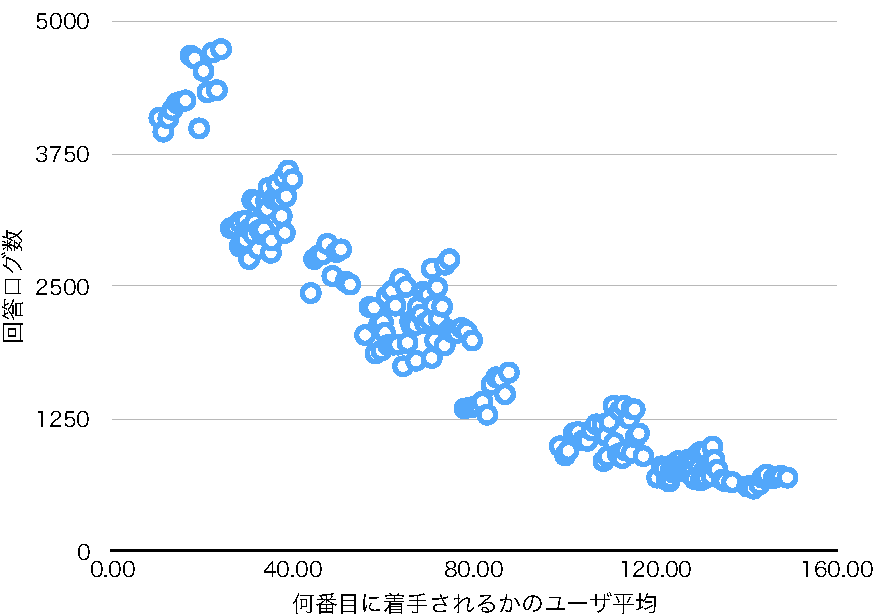
\includegraphics[width=200pt, height=150pt]{./img/stats_s5_soc.pdf}
	\caption{小学5年社会の平均着手順と回答ログ数のXYプロット}
	\label{fig:stats_s5_soc}
\endminipage\hfill
\end{center}
\end{figure}
小学5年社会では,主に,首都,地球儀,緯度経度,山地山脈,気候,平野,海流,特産物,農林水産業,輸出入,自給率,自動車などの社会基盤や社会問題に関する基本内容が扱われる.
図\ref{fig:qa_s5_soc}に,問題と回答選択肢の例を示す.
図の問題は社会問題のうち近年しばしば議論されている個人情報とインターネットに関する問題であり,
その回答を選択肢のなかから選択する,という回答形式である.
次に,各問題について何番目に着手されるかの平均値と回答ログ数の関係を図\ref{fig:stats_s5_soc}に示す.
全体として,概ね500件以上の回答ログ数があり,回答ログの分布については小学4年の社会と概ね同じである.


\subsubsection{小学5年算数}
\begin{figure}[ht]
\begin{center}
\minipage{0.48\textwidth}
	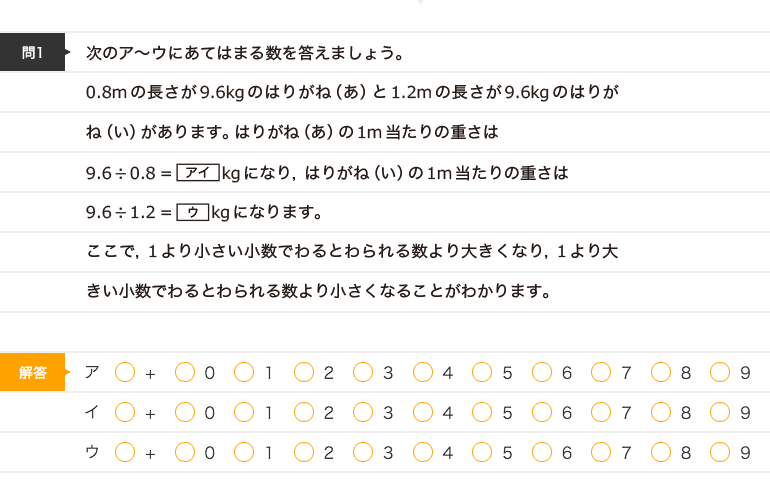
\includegraphics[width=200pt, height=150pt]{./img/qa_s5_mat2.png}
	\caption{小学5年算数の問題と回答選択肢の例}
	\label{fig:qa_s5_mat}
\endminipage\hfill
\minipage{0.48\textwidth}
	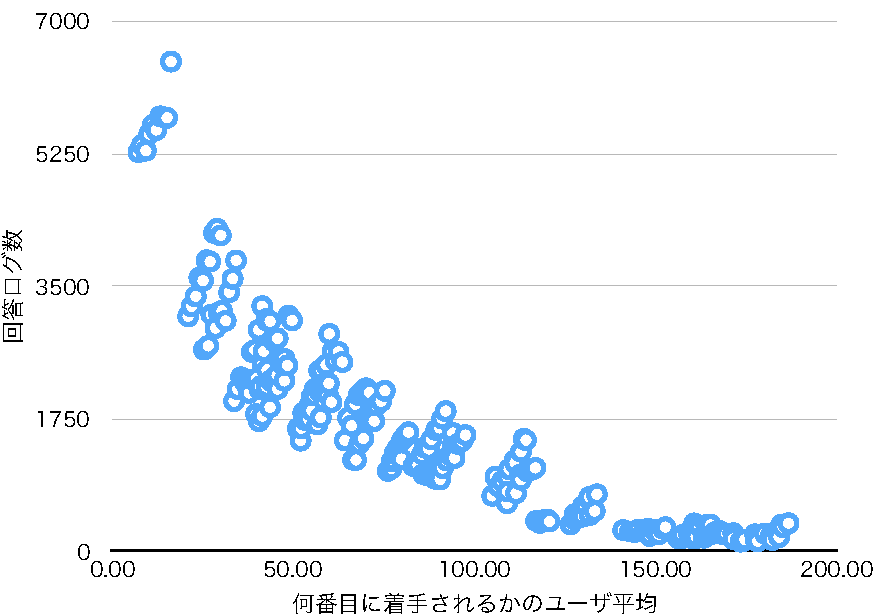
\includegraphics[width=200pt, height=150pt]{./img/stats_s5_mat.pdf}
	\caption{小学5年算数の平均着手順と回答ログ数のXYプロット}
	\label{fig:stats_s5_mat}
\endminipage\hfill
\end{center}
\end{figure}
小学5年算数では,主に,整数,約数,倍数,平行四辺形,内角,外角,展開図,円,柱,などの基本内容が扱われる.
図\ref{fig:qa_s5_mat}に,問題と回答選択肢の例を示す.
図の問題は小数の割り算に関する問題であり,
その回答を選択肢のなかから選択する,という回答形式である.
特に,回答の桁数が指定されているだけで,回答欄への自由記述に近い回答形式である.
次に,各問題について何番目に着手されるかの平均値と回答ログ数の関係を図\ref{fig:stats_s5_mat}に示す.
最後の方の問題他の問題と比べると回答ログ数がかなり小さい.


\subsubsection{小学6年社会}
\begin{figure}[ht]
\begin{center}
\minipage{0.48\textwidth}
	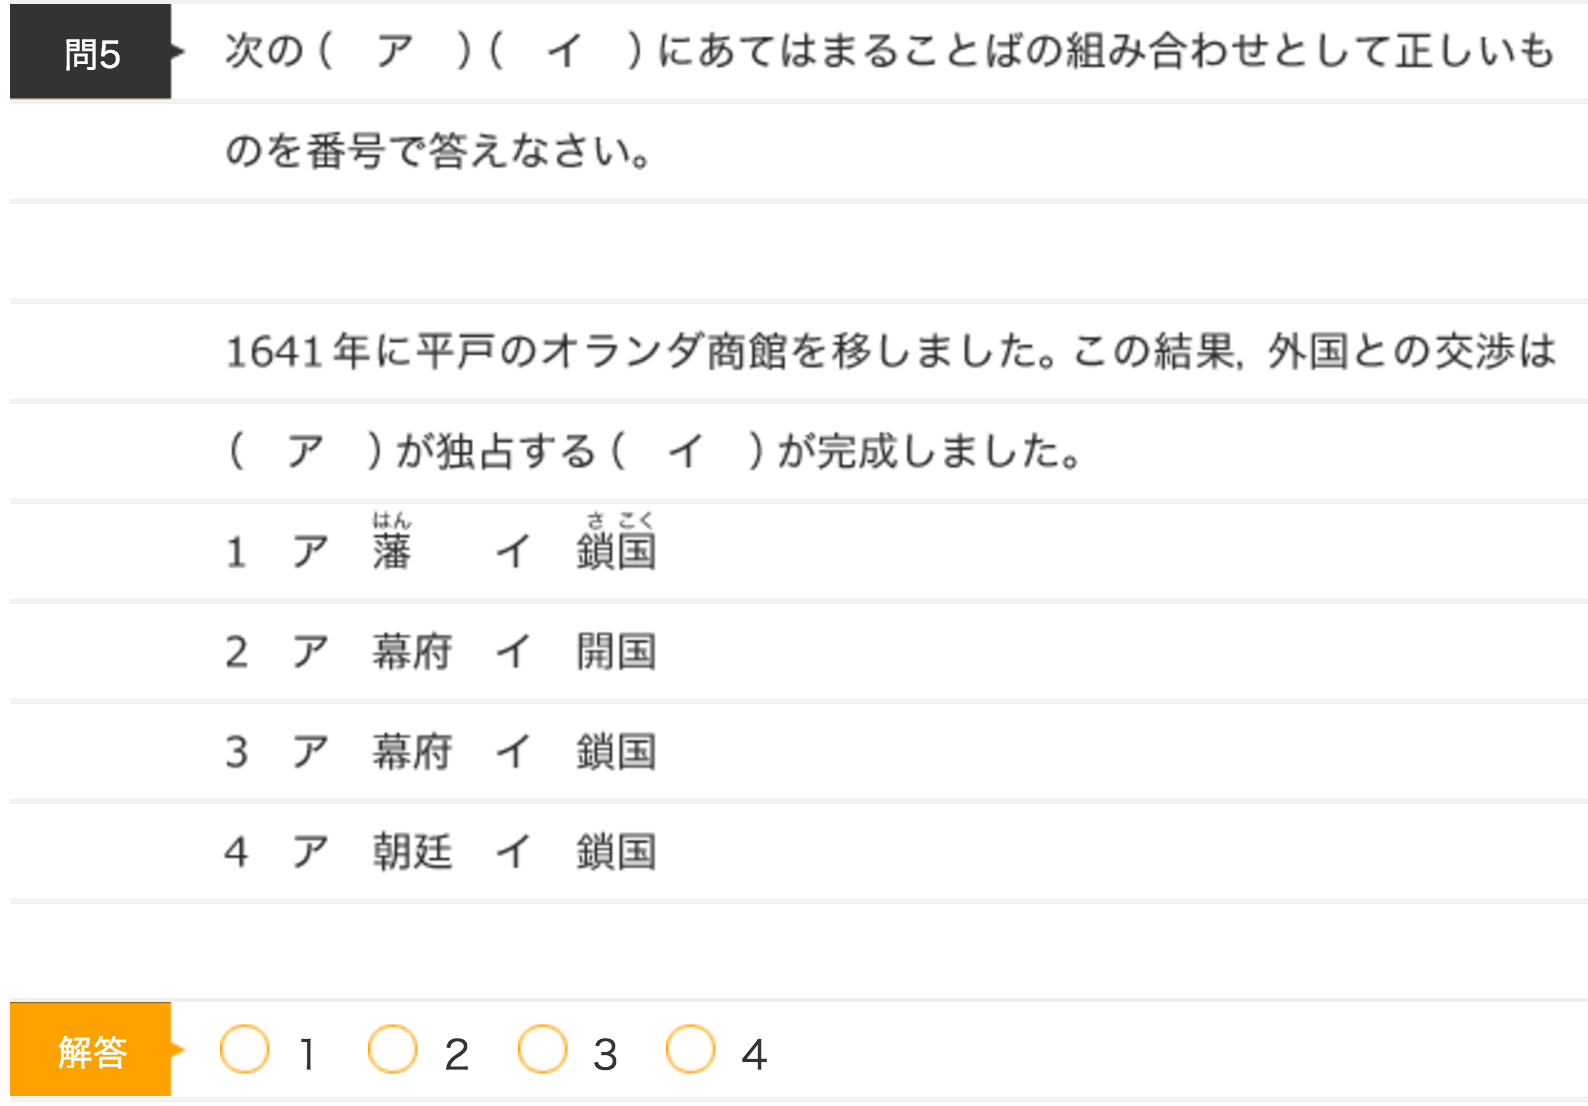
\includegraphics[width=200pt, height=150pt]{./img/qa_s6_soc.png}
	\caption{小学6年社会の問題と回答選択肢の例}
	\label{fig:qa_s6_soc}
\endminipage\hfill
\minipage{0.48\textwidth}
	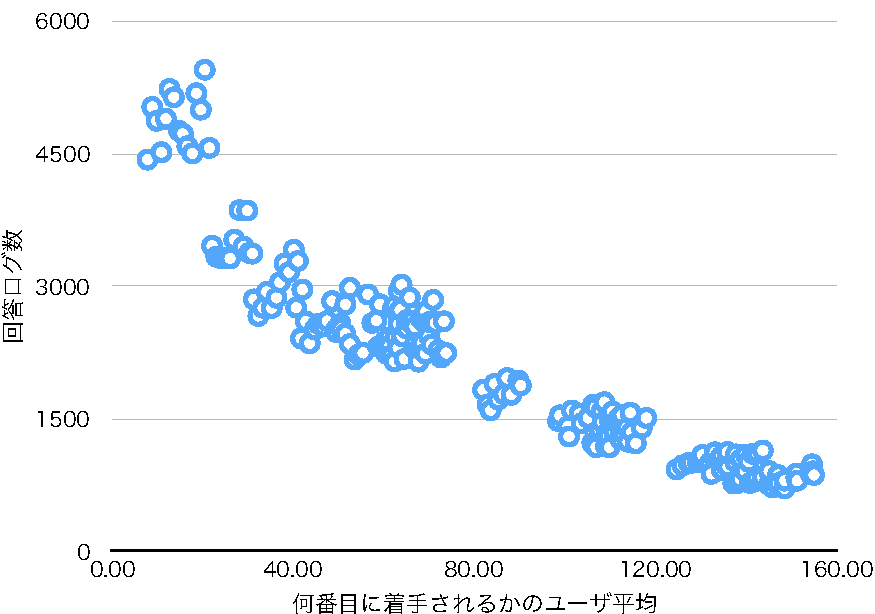
\includegraphics[width=200pt, height=150pt]{./img/stats_s6_soc.pdf}
	\caption{小学6年社会の平均着手順と回答ログ数のXYプロット}
	\label{fig:stats_s6_soc}
\endminipage\hfill
\end{center}
\end{figure}
小学6年社会では,主に,旧石器・縄文・弥生・古墳時代から昭和時代までの幅広い期間の歴史に関する内容が扱われる.
図\ref{fig:qa_s6_soc}に,問題と回答選択肢の例を示す.
図の問題は江戸時代の鎖国に関する問題であり,
その回答を選択肢のなかから選択する,という回答形式である.
次に,各問題について何番目に着手されるかの平均値と回答ログ数の関係を図\ref{fig:stats_s6_soc}に示す.
小学4年,小学5年の社会と同様に,概ね一定の割合で後半の問題の回答ログ数が減っていっていることがわかる.



\subsubsection{小学6年算数}
\begin{figure}[ht]
\begin{center}
\minipage{0.48\textwidth}
	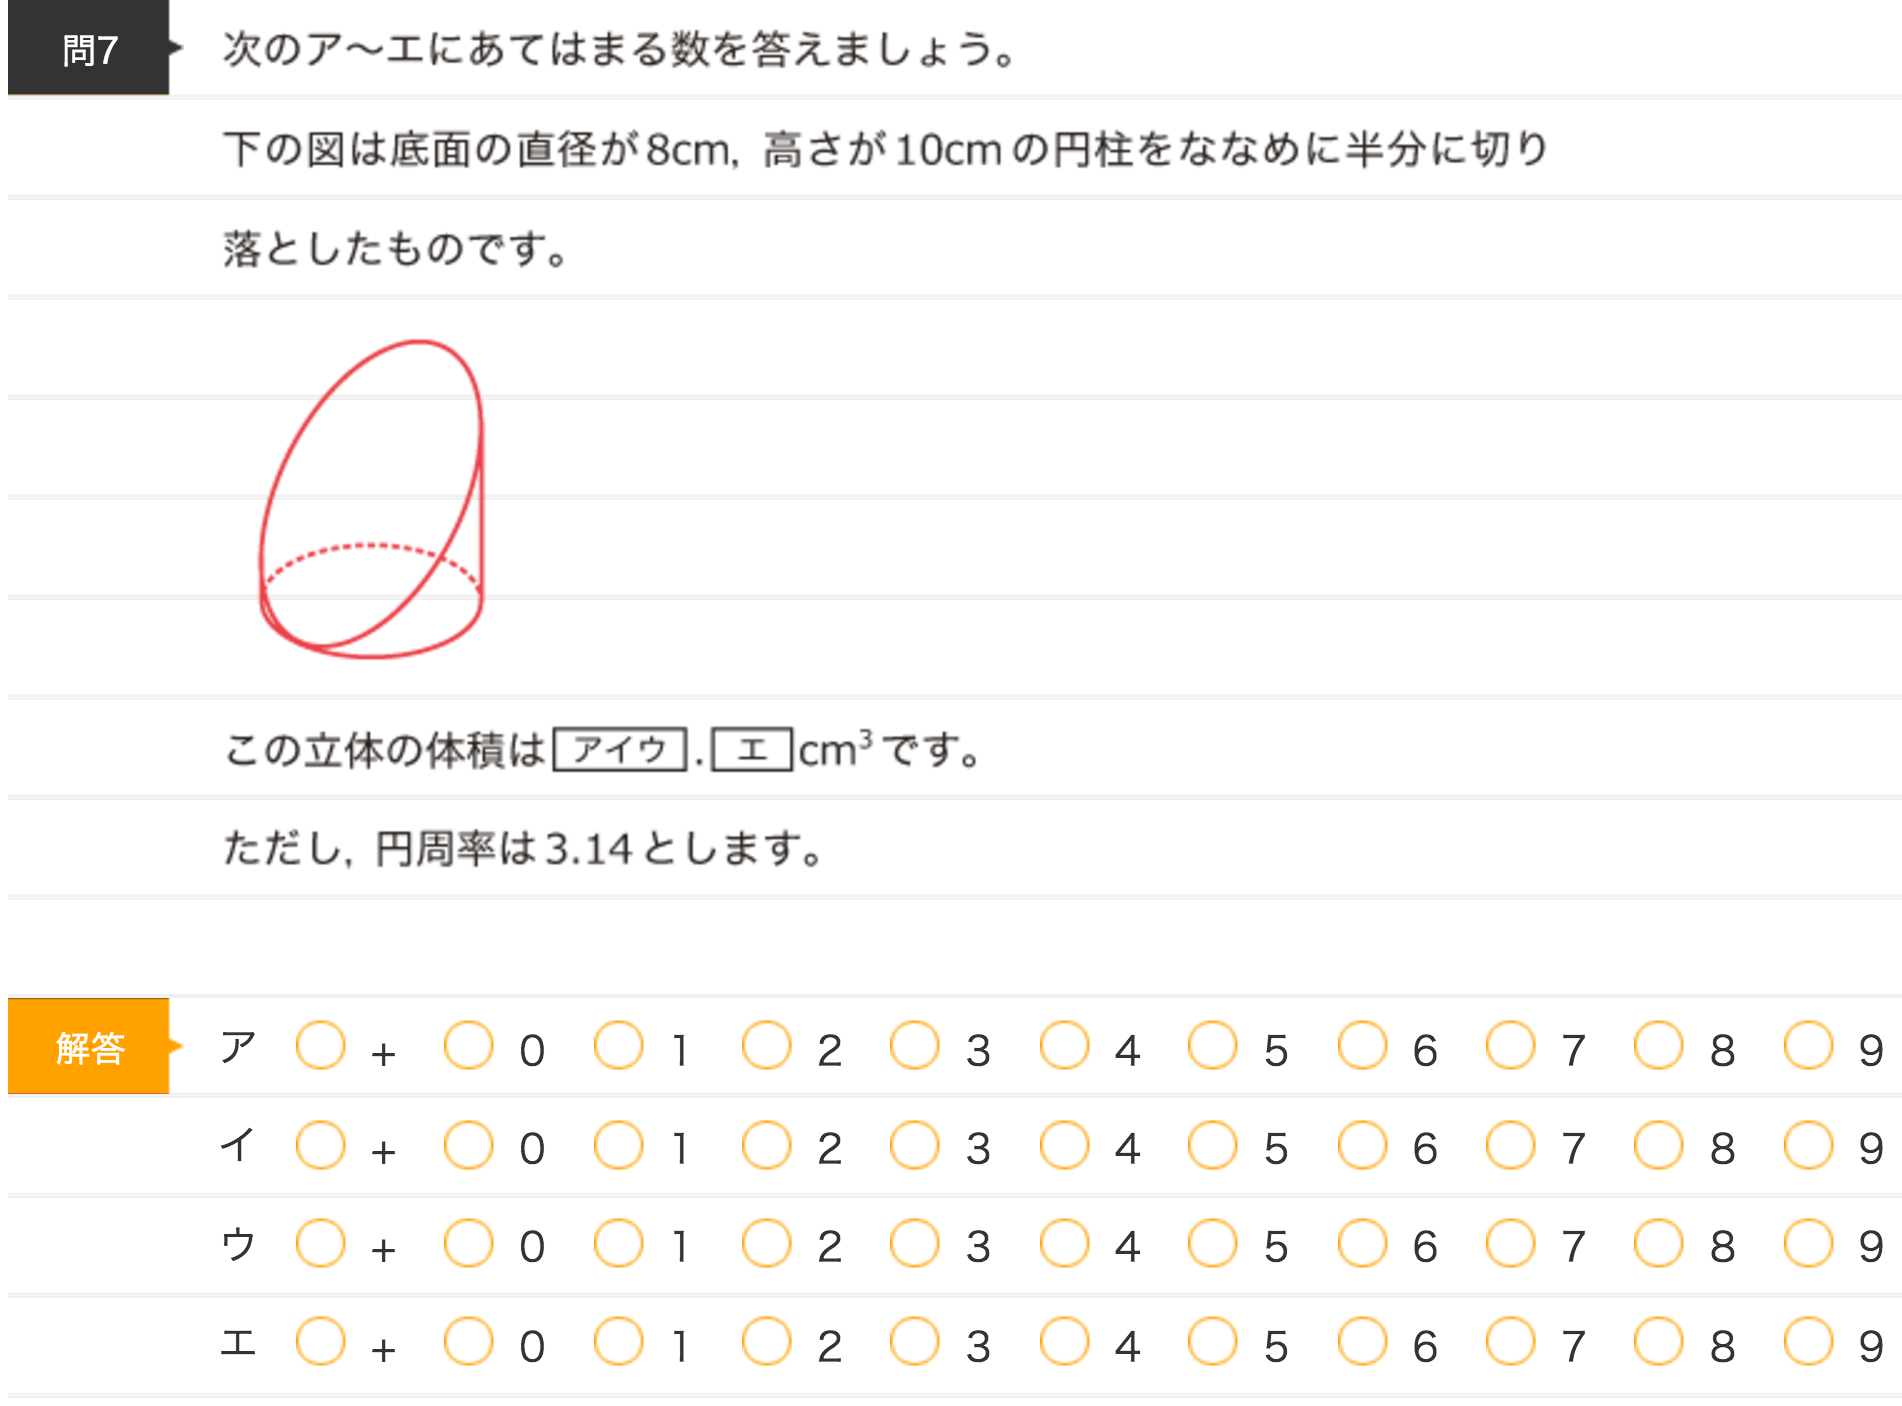
\includegraphics[width=200pt, height=150pt]{./img/qa_s6_mat.png}
	\caption{小学6年算数の問題と回答選択肢の例}
	\label{fig:qa_s6_mat}
\endminipage\hfill
\minipage{0.48\textwidth}
	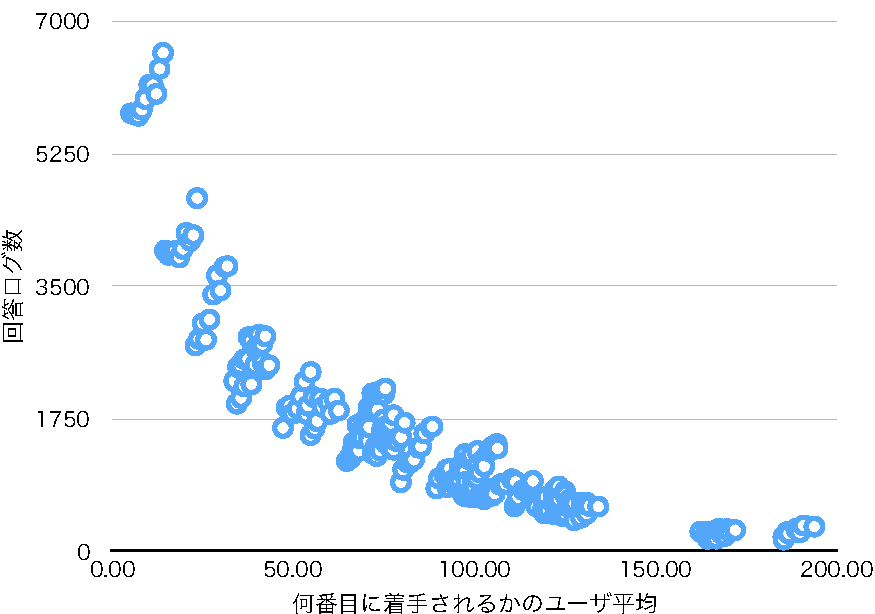
\includegraphics[width=200pt, height=150pt]{./img/stats_s6_mat.pdf}
	\caption{小学6年算数の平均着手順と回答ログ数のXYプロット}
	\label{fig:stats_s6_mat}
\endminipage\hfill
\end{center}
\end{figure}
小学6年算数では,主に,ならべ方と組み合わせ方,倍と割合,円の面積,分数のかけ算,分数のわり算,小数と分数の計算,拡大図と縮図,文字と式,比とその利用,比例と反比例,点対称,立体の体積,線対称,資料の調べ方,速さ,量と単位の基本内容が扱われる.
図\ref{fig:qa_s6_mat}に,問題と回答選択肢の例を示す.
図の問題は立体の体積のうち特に円柱の体積に関する問題であり,
その回答を選択肢のなかから選択する,という回答形式である.
特に,回答の桁数が指定されているだけで,回答欄への自由記述に近い回答形式である.
次に,各問題について何番目に着手されるかの平均値と回答ログ数の関係を図\ref{fig:stats_s6_mat}に示す.
小学4年,小学5年の算数と比べ,分布が下に凸の形になっており,
最初の方の問題への回答ログの偏りが大きいことが分かる.


\subsubsection{中学1年数学}
\begin{figure}[ht]
\begin{center}
\minipage{0.48\textwidth}
	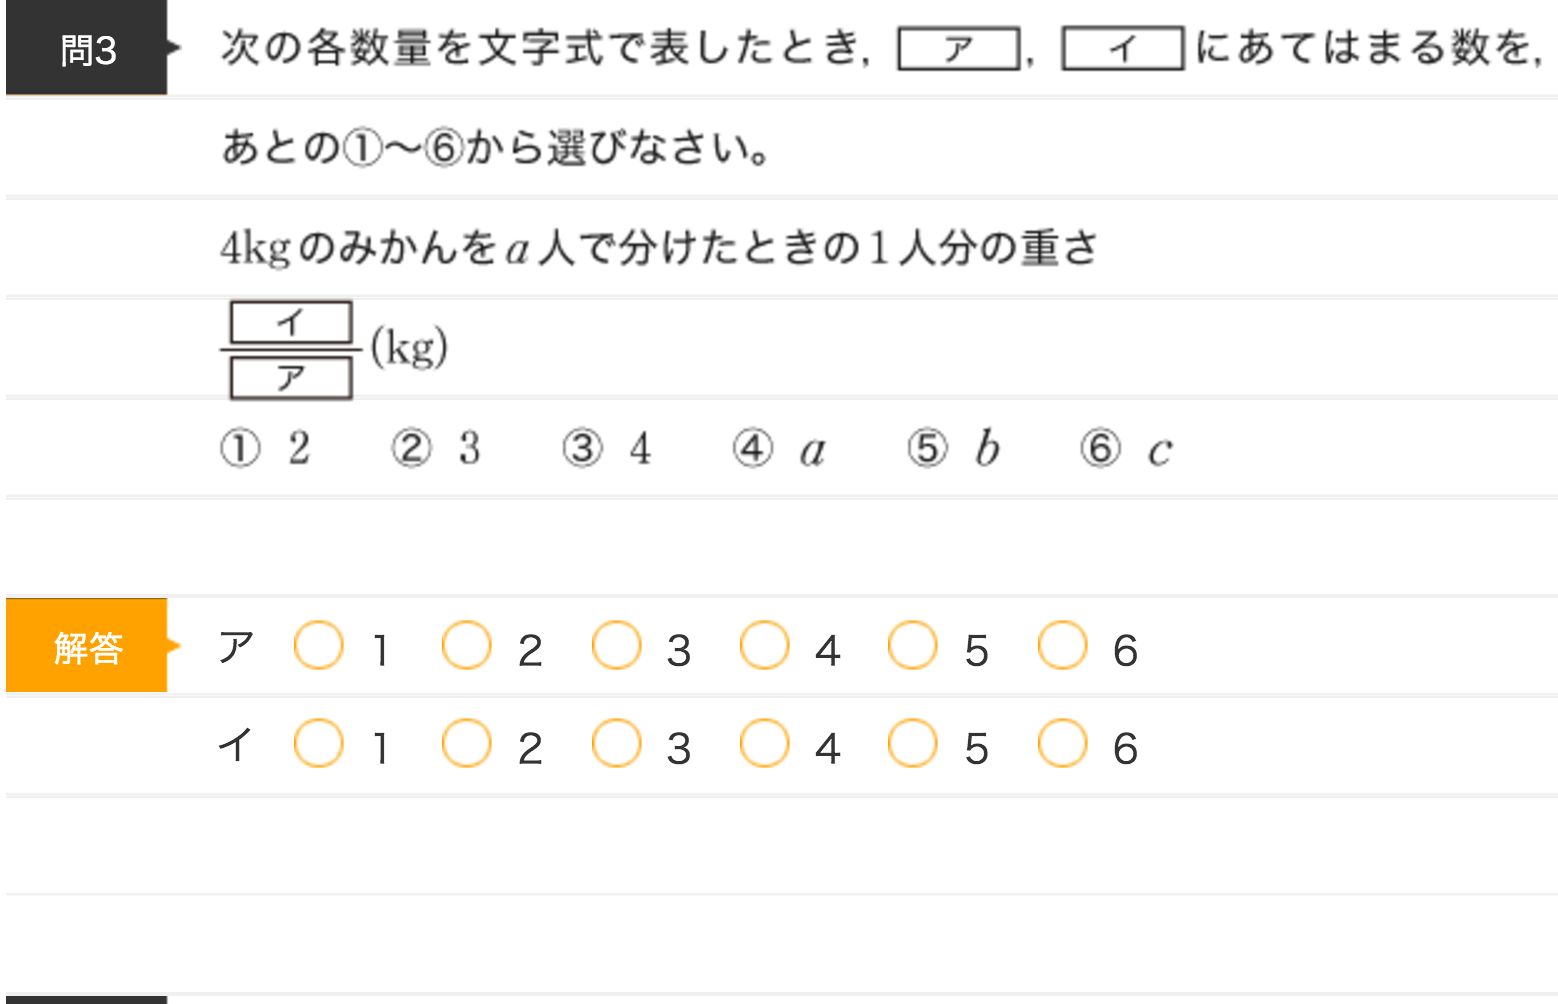
\includegraphics[width=200pt, height=150pt]{./img/qa_c1_mat.png}
	\caption{中学1年数学の問題と回答選択肢の例}
	\label{fig:qa_c1_mat}
\endminipage\hfill
\minipage{0.48\textwidth}
	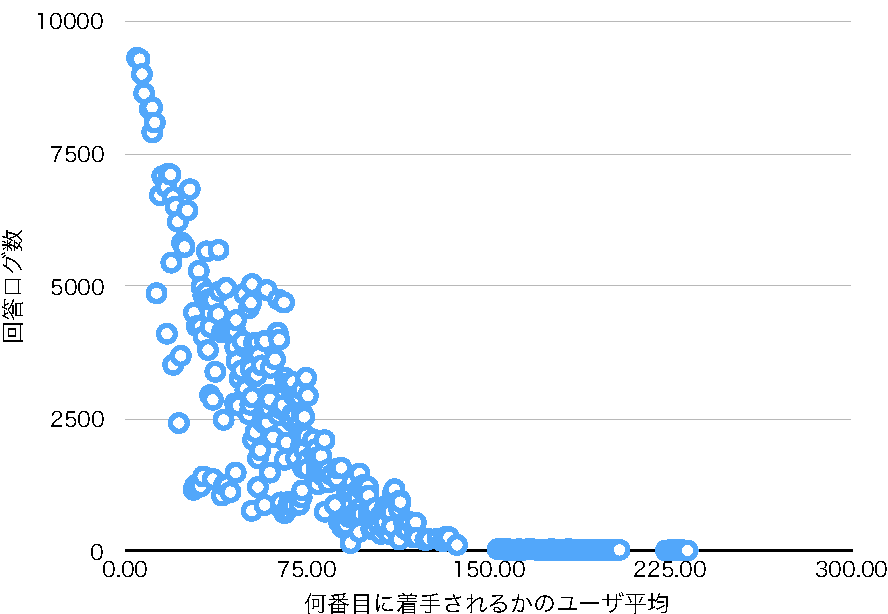
\includegraphics[width=200pt, height=150pt]{./img/stats_c1_mat.pdf}
	\caption{中学1年数学の平均着手順と回答ログ数のXYプロット}
	\label{fig:stats_c1_mat}
\endminipage\hfill
\end{center}
\end{figure}
中学1年数学では,主に,
1次式,1次方程式,2平面の関係 面の動き,代入と式の値,作図のしかた,円,反比例,図形の移動,対称移動,平面上の2直線,度数の分布,座標,数の集合と四則計算,文字式の活用,方程式,正負の数の利用,比と比例式,立体の体積,角錐と円錐
などに関する内容が扱われる.
図\ref{fig:qa_c1_mat}に,問題と回答選択肢の例を示す.
図の問題は文字式を活用した問題であり,
その回答を選択肢のなかから選択する,という回答形式である.
次に,各問題について何番目に着手されるかの平均値と回答ログ数の関係を図\ref{fig:stats_c1_mat}に示す.
回答ログは最初の方の問題に大きく偏っており,特に後半の一部は数十程度のログしかないことが分かる.


\subsubsection{中学2年数学}
\begin{figure}[ht]
\begin{center}
\minipage{0.48\textwidth}
	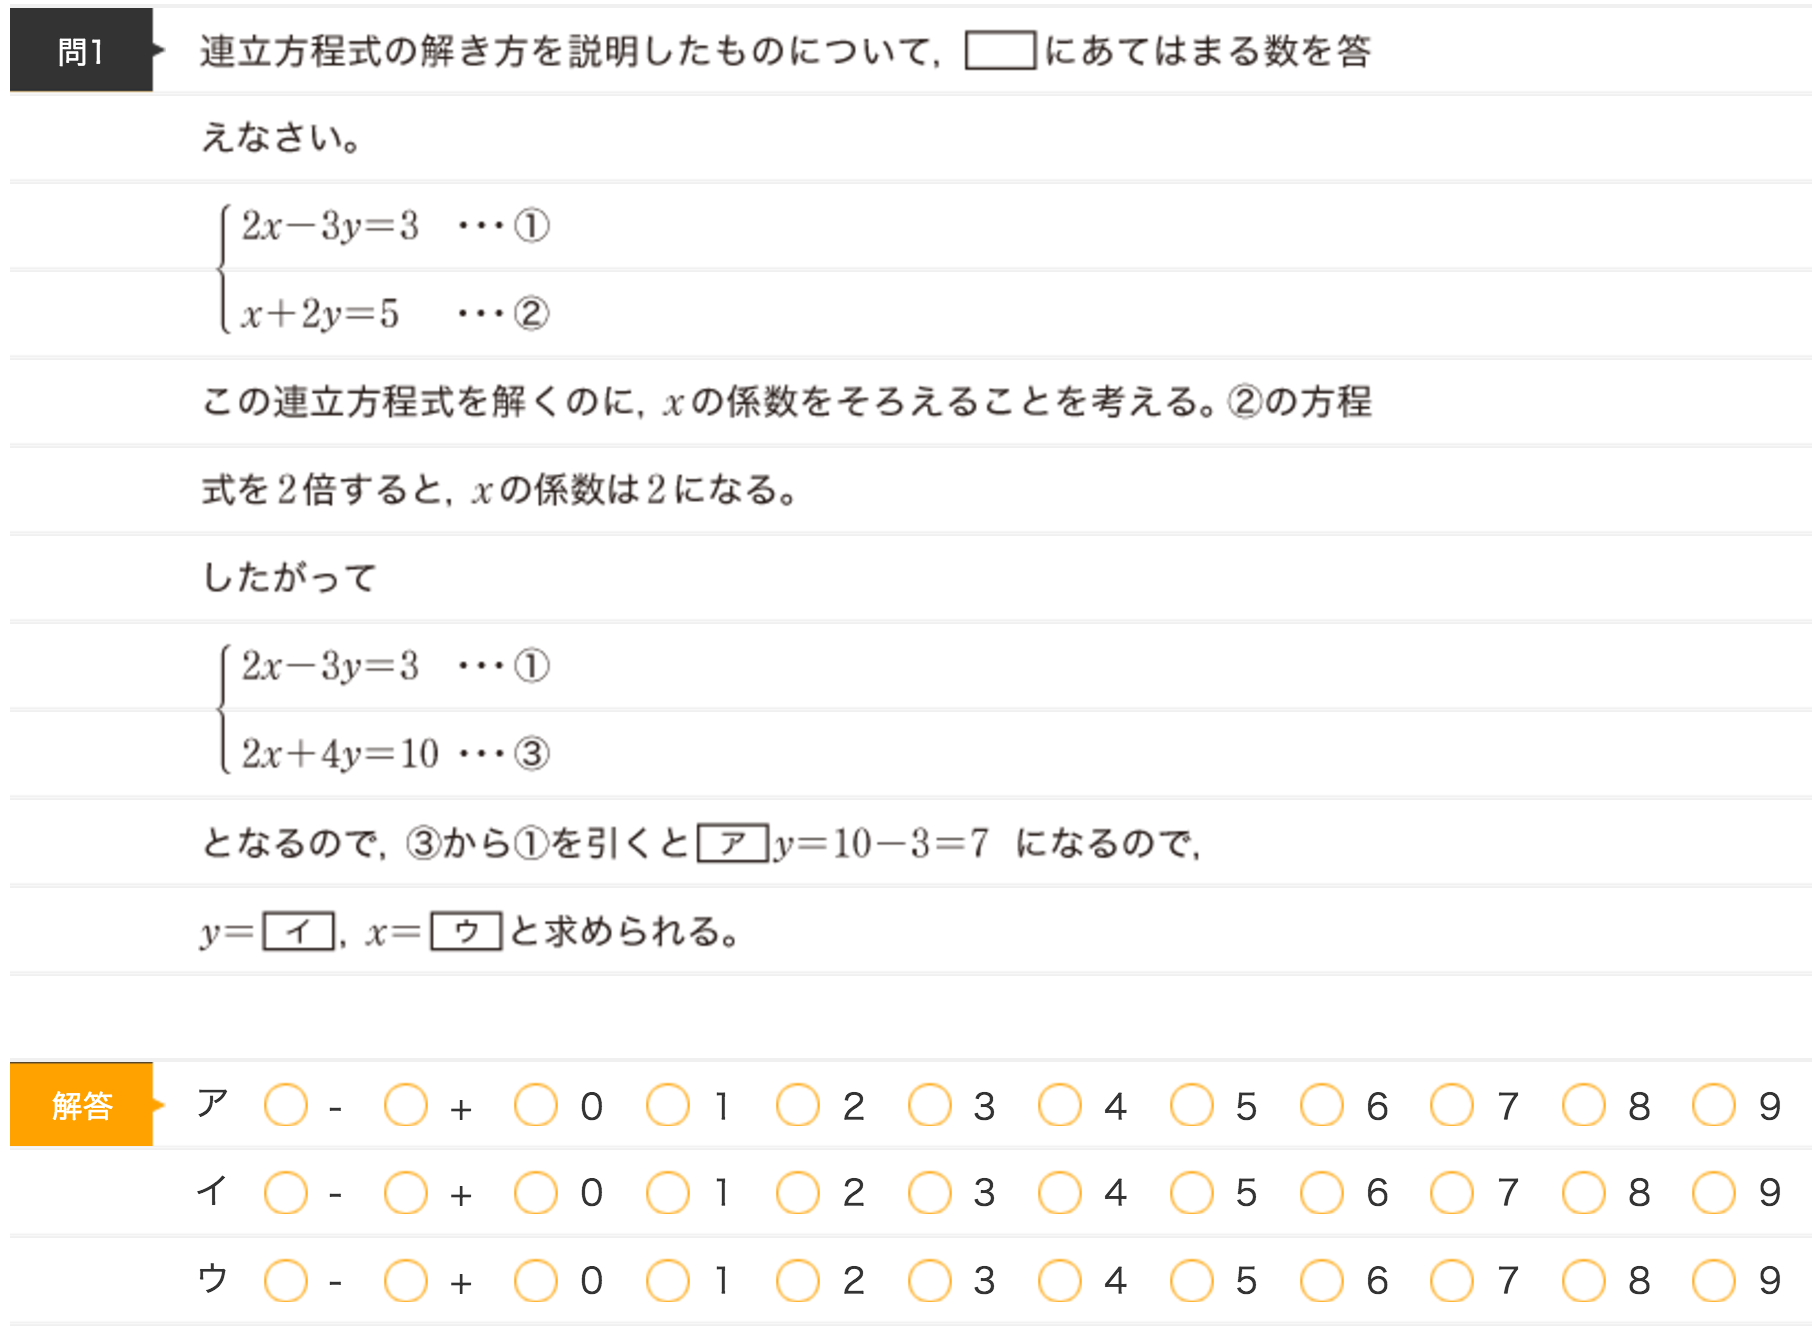
\includegraphics[width=200pt, height=150pt]{./img/qa_c2_mat.png}
	\caption{中学2年数学の問題と回答選択肢の例}
	\label{fig:qa_c2_mat}
\endminipage\hfill
\minipage{0.48\textwidth}
	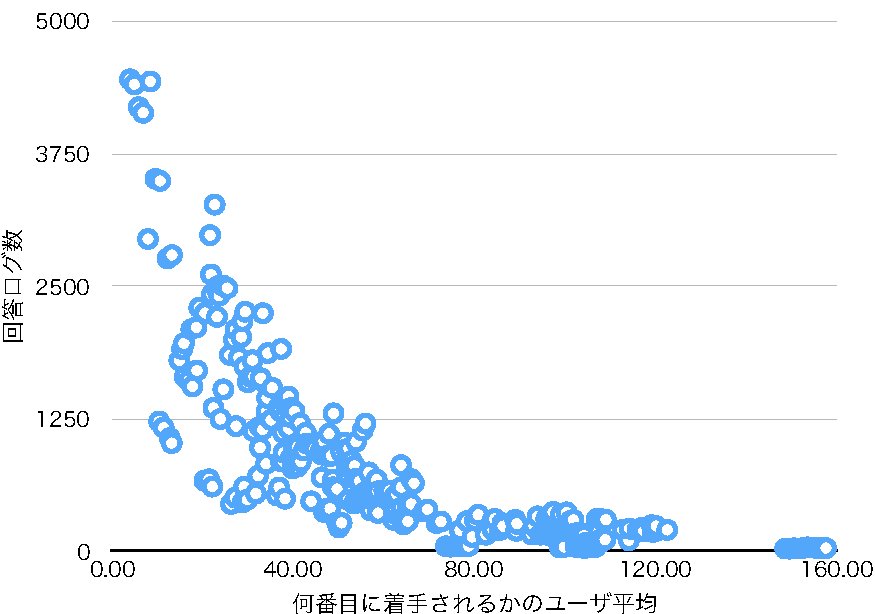
\includegraphics[width=200pt, height=150pt]{./img/stats_c2_mat.pdf}
	\caption{中学2年数学の平均着手順と回答ログ数のXYプロット}
	\label{fig:stats_c2_mat}
\endminipage\hfill
\end{center}
\end{figure}
中学2年数学では,主に,
1次方程式,1次関数,三角形の合同条件,二等辺三角形,仮定と結論,単項式と多項式,合同な三角形,平行四辺形,証明,連立方程式
などを扱う.
扱う内容は中学1年数学のデータセットのものと概ね同様であるが,難易度が高い.
図\ref{fig:qa_c2_mat}に,問題と回答選択肢の例を示す.
図の問題は数連立方程式に関する問題であり,
その回答を選択肢のなかから選択する,という回答形式である.
次に,各問題について何番目に着手されるかの平均値と回答ログ数の関係を図\ref{fig:stats_c2_mat}に示す.
グラフの外見は中学1年数学に近いが,回答ログ数のスケールが半分程度である.
また,一部の問題については,ログが数十程度と他と比べると非常に少なくなっている.


\subsubsection{中学3年数学}
\begin{figure}[ht]
\begin{center}
\minipage{0.48\textwidth}
	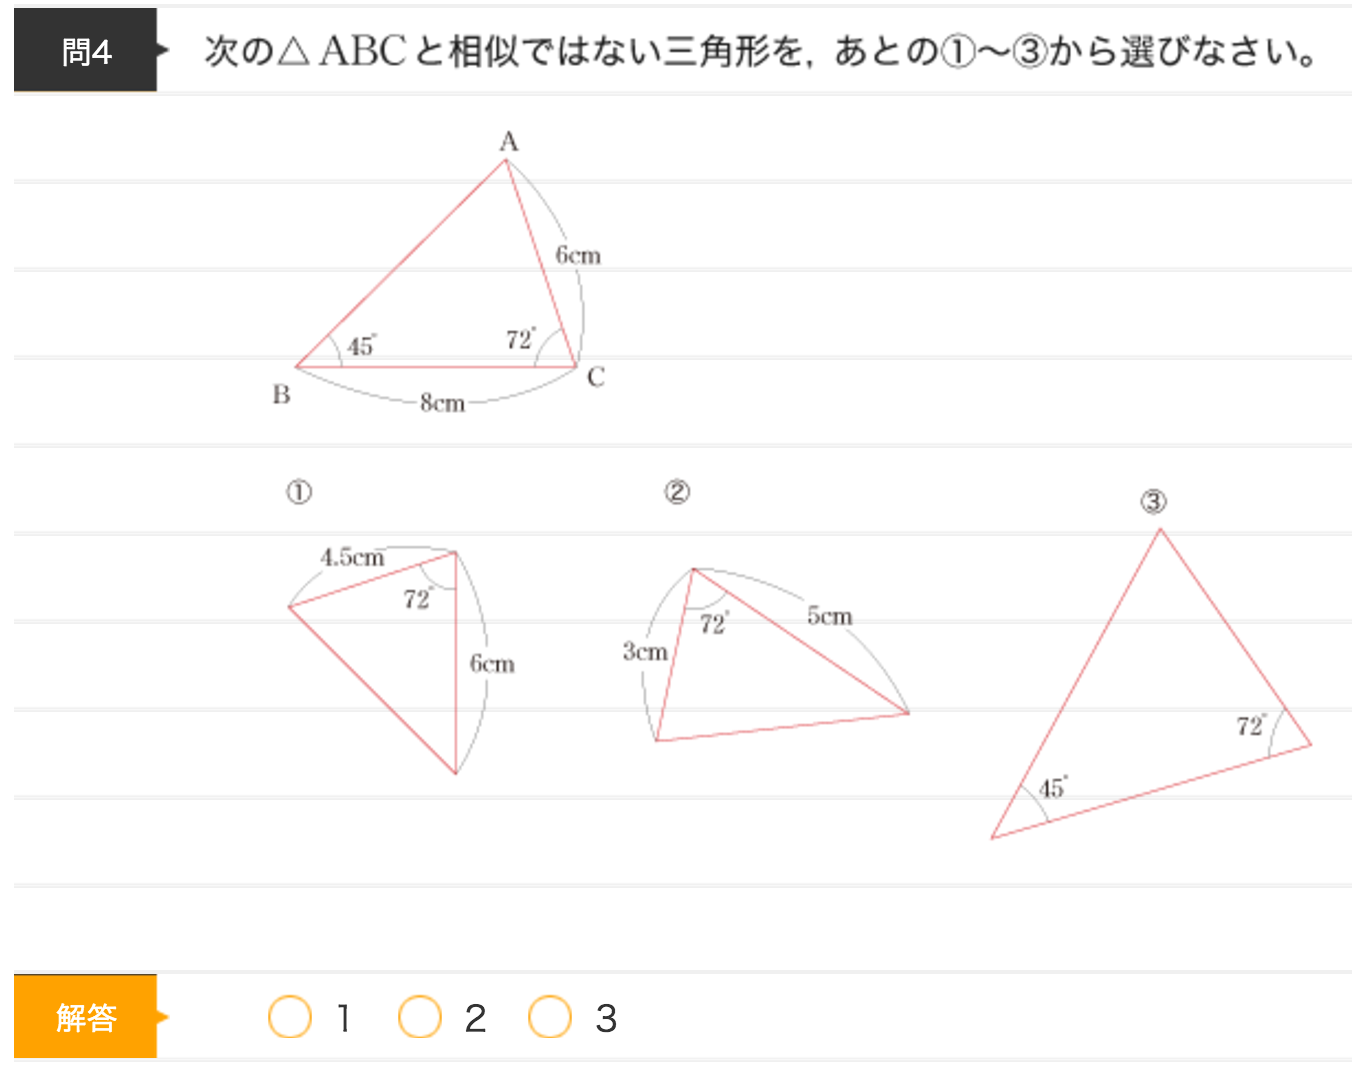
\includegraphics[width=200pt, height=150pt]{./img/qa_c3_mat.png}
	\caption{中学3年数学の問題と回答選択肢の例}
	\label{fig:qa_c3_mat}
\endminipage\hfill
\minipage{0.48\textwidth}
	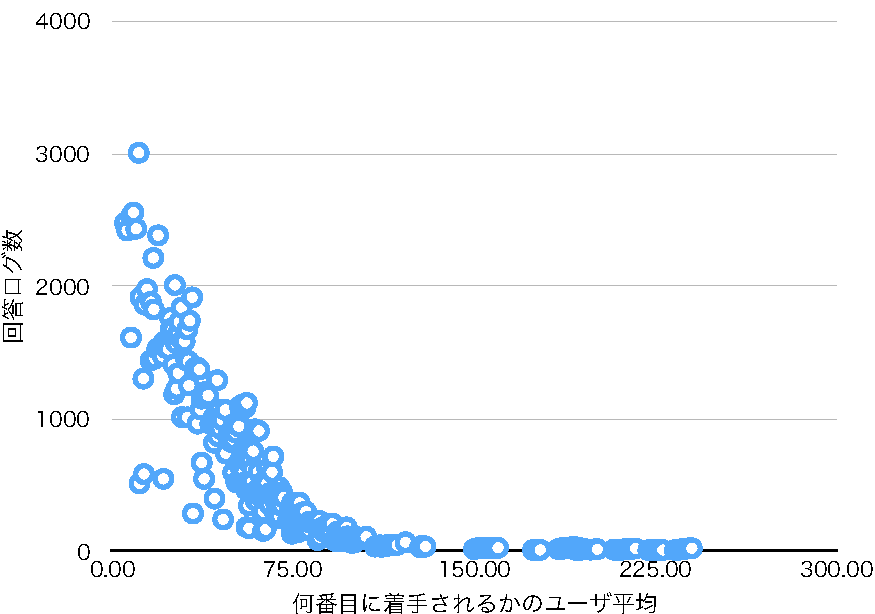
\includegraphics[width=200pt, height=150pt]{./img/stats_c3_mat.pdf}
	\caption{中学3年数学の平均着手順と回答ログ数のXYプロット}
	\label{fig:stats_c3_mat}
\endminipage\hfill
\end{center}
\end{figure}
中学3年数学では,
たすき掛け,一次関数,三平方の定理,中点連結定理,乱数表,二次方程式,二次関数,円の面積,円周角,分配法則,回転体の体積,因数分解,増加関数,変域,外接円,媒介変数,展開,平方完成,平方根,平行線,循環小数,指数,接線の定義,放物線,文字式,有理数,根号,標本調査,母集団,減少関数,無理数,相似の三角形,相似比,立方体,等差数列の和,約数,素因数分解,素数,解と係数の関係
などの内容が扱われる.
図\ref{fig:qa_c3_mat}に,問題と回答選択肢の例を示す.
図の問題は図形のうち相似の三角形に関する問題であり,
その回答を選択肢のなかから選択する,という回答形式である.
次に,各問題について何番目に着手されるかの平均値と回答ログ数の関係を図\ref{fig:stats_c3_mat}に示す.
グラフの外観は中学2年数学に類似しているが,
後半の問題の回答ログ数は非常に少ない.


\subsubsection{中学地理}
\begin{figure}[ht]
\begin{center}
\minipage{0.48\textwidth}
	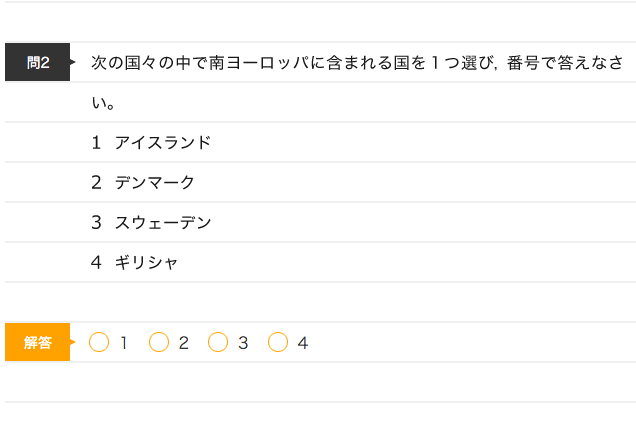
\includegraphics[width=200pt, height=150pt]{./img/qa_c_geo2.png}
	\caption{中学地理の問題と回答選択肢の例}
	\label{fig:qa_c_geo}
\endminipage\hfill
\minipage{0.48\textwidth}
	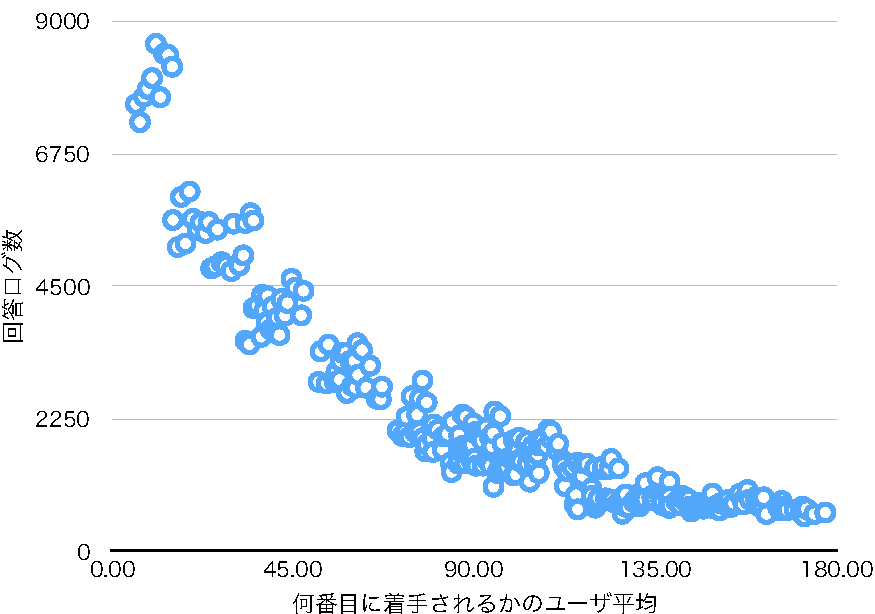
\includegraphics[width=200pt, height=150pt]{./img/stats_c_geo.pdf}
	\caption{中学地理の平均着手順と回答ログ数のXYプロット}
	\label{fig:stats_c_geo}
\endminipage\hfill
\end{center}
\end{figure}
中学地理では,主に,
アジア,アフリカ,オセアニア,ヨーロッパ,北アメリカ,南アメリカ,世界と日本の関係,世界の地域区分と特色,世界の衣食住・宗教,地域の調査,日本の地域区分,日本の工業と商業・サービス業,日本の農林水産業,東北地方,近畿地方,関東地方,中部地方,九州地方,北海道地方,中国・四国地方
などが地域や地域の性質,地域間の関係性が扱われる.
図\ref{fig:qa_c_geo}に,問題と回答選択肢の例を示す.
図の問題はヨーロッパに関する問題であり,
その回答を選択肢のなかから選択する,という回答形式である.
次に,各問題について何番目に着手されるかの平均値と回答ログ数の関係を図\ref{fig:stats_c_geo}に示す.
全体として,概ね500以上の回答ログ数があり,前半の問題から後半の問題にかけてほぼ線形に回答ログ数が減少している.


\subsubsection{中学歴史}
\begin{figure}[ht]
\begin{center}
\minipage{0.48\textwidth}
	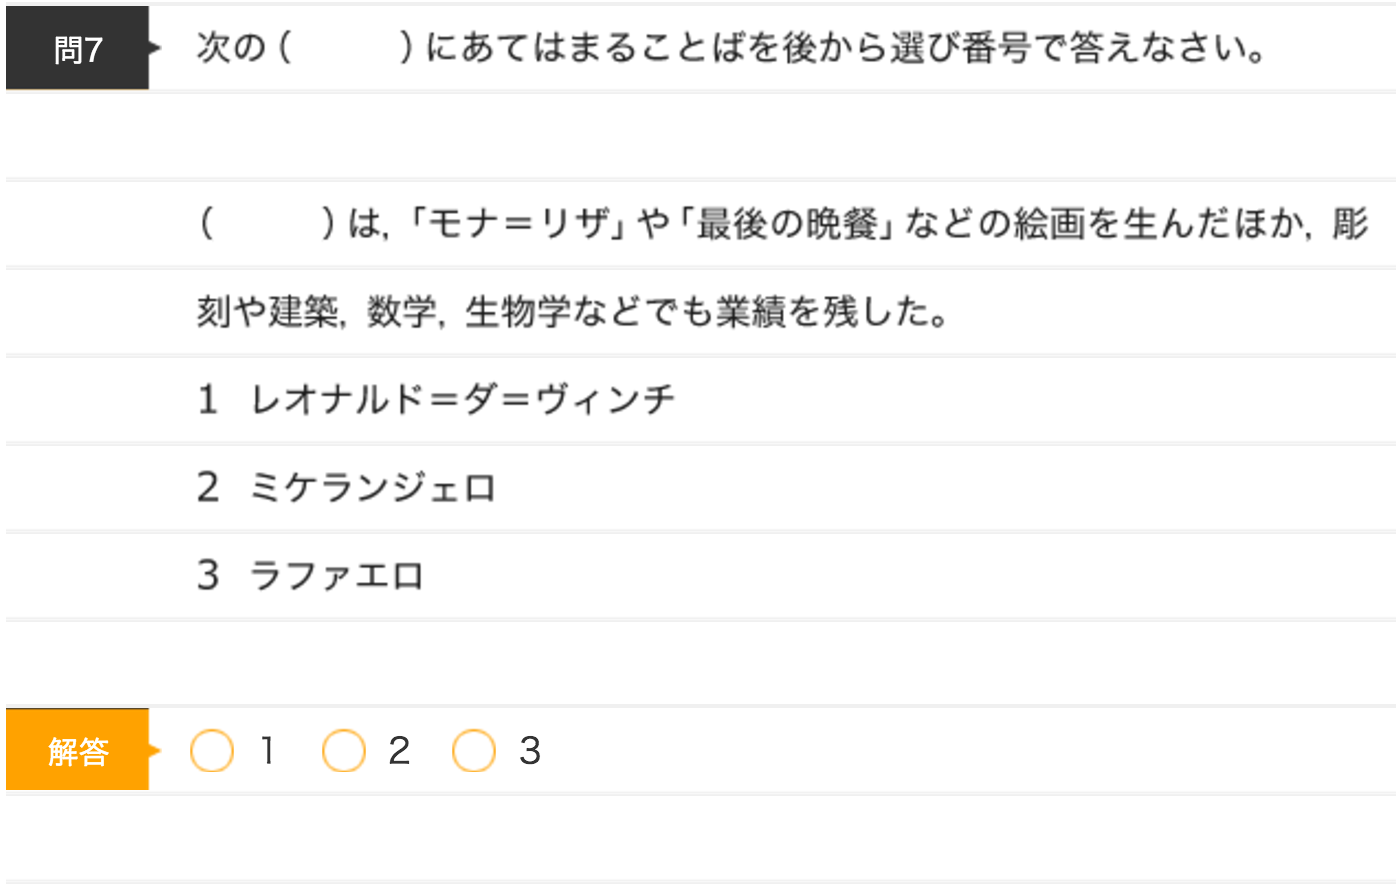
\includegraphics[width=200pt, height=150pt]{./img/qa_c_his.png}
	\caption{中学歴史の問題と回答選択肢の例}
	\label{fig:qa_c_his}
\endminipage\hfill
\minipage{0.48\textwidth}
	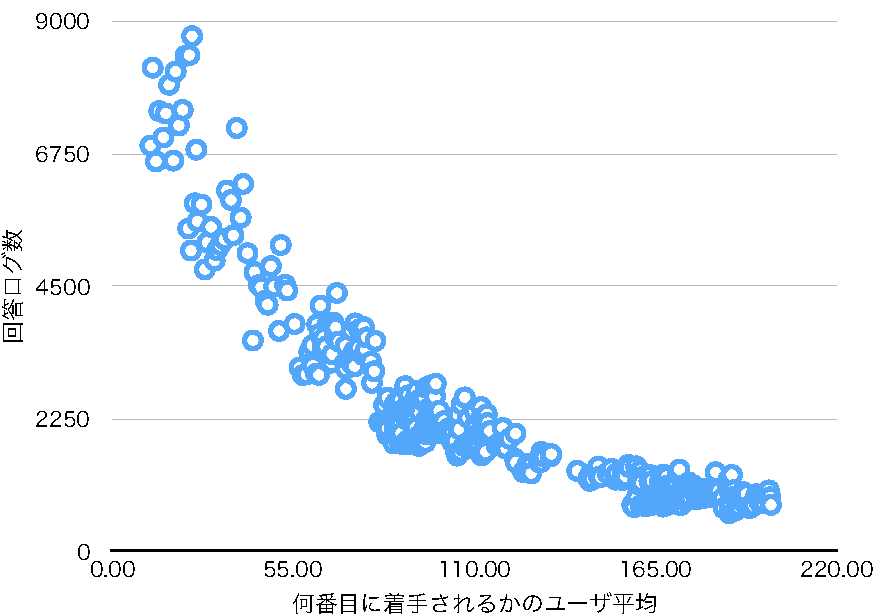
\includegraphics[width=200pt, height=150pt]{./img/stats_c_his.pdf}
	\caption{中学歴史の平均着手順と回答ログ数のXYプロット}
	\label{fig:stats_c_his}
\endminipage\hfill
\end{center}
\end{figure}
中学歴史では,主に,
ルネサンスと大航海時代,世界恐慌と国際情勢の悪化,世界文明の発生,国際協調体制,第一次世界大戦とロシア革命,欧米の市民革命と産業革命,旧石器・縄文・弥生時代,安土桃山時代,大和時代,奈良時代,平安時代,鎌倉時代,室町時代,江戸時代,明治時代,昭和時代,大正時代,平成時代
,など内容が扱われる.
図\ref{fig:qa_c_his}に,問題と回答選択肢の例を示す.
図の問題はルネサンスと大航海時代に関する問題と推察される.
その回答を選択肢のなかから選択する,という回答形式である.
次に,各問題について何番目に着手されるかの平均値と回答ログ数の関係を図\ref{fig:stats_c_his}に示す.
全体として,概ね500以上の回答ログ数があり,前半の問題から後半の問題にかけてほぼ線形に回答ログ数が減少している.
外観は中学地理と概ね合致している.


以上,個々のデータセットおよびデータが収集された講座を具体的に説明した.
具体的な内容から,
地理と歴史に関する5講座(小学4年社会,小学5年社会,小学6年社会,中学地理,中学歴史)のデータセットが
どちらかというと,宣言的知識の獲得を主目的としているデータセットであり,
算数や数学に関する6講座(小学4年算数,小学5年算数,小学6年算数,中学1年数学,中学2年数学,中学3年数学)のデータセットが
どちらかというと,手続き的知識の獲得を主目的としているデータセットであることが分かる.


また,データセットの一部の問題については他の問題と比べてログ数が数十程度と少なかったが,
それでも数十程度のログデータがあり,
そうした問題が一部に限られていることから
知識構造を抽出できると考え,このまま全ての問題をデータセットに利用する.


\vvspace
以上,データセットについて述べた.
次章では,実験について述べる.

